\section{Updated Project Timetable}
\label{sec:timetable}

My internship at isMOOD started
on \emph{March 18\textsuperscript{th}, 2019}
and was completed 
on \emph{June 17\textsuperscript{th}, 2019}.
The time duration of all activities
described in Section~\ref{sec:results}
is depicted in the following timetable:

\begin{table}[ht]
\caption{\label{tab:timetable}Timetable}
\centering
\begin{tabular}{ |c|c| }
 \hline
 \textbf{Activity} & \textbf{Duration} \\ 
 \hline
 Training at Business Team & 1 week \\
 \hline
 Research Conduction & 2 weeks \\ 
 \hline
 Database Construction & 8 weeks \\ 
 \hline
 Algorithm Development \& Testing & 4 weeks \\
 \hline
\end{tabular}
\end{table}

The timeline of the abovementioned activities
is depicted in the following figure (Gantt chart)
using \emph{week} as time unit:

\begin{figure}[ht]
\centering
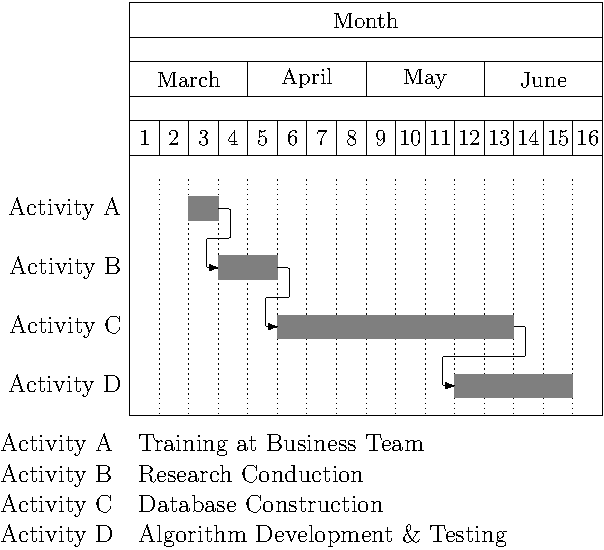
\includegraphics{gantt-chart.eps}
\caption{Gantt Chart}
\label{fig:gantt-chart}
\end{figure}

% DOES NOT COMPILE PROPERLY
% \noindent
% \begin{ganttchart}[vgrid, bar/.style={fill=gray!100}] {1}{16}
% \gantttitle{Month}{16} \\
% \gantttitle{March}{4} 
% \gantttitle{April}{4} 
% \gantttitle{May}{4} 
% \gantttitle{June}{4} \\
% \gantttitlelist{1,...,16}{1} \\
% \ganttbar{Activity A}{3}{3} \\ 
% \ganttbar{Activity B}{4}{5} \\
% \ganttbar{Activity C}{6}{13} \\
% \ganttbar{Activity D}{12}{15} 
% \ganttlink{elem0}{elem1}
% \ganttlink{elem1}{elem2} 
% \ganttlink{elem2}{elem3}
% \end{ganttchart}
% \medskip
% 
% \noindent
% \begin{tabularx}\linewidth{@{}lX@{}}
%   Activity A & Training at Business Team \\
%   Activity B & Research Conduction\\
%   Activity C & Database Construction\\
%   Activity D & Algorithm Development \& Testing
% \end{tabularx}
